\chapter{Introduction}
With the advent of quantum mechanics in the early twentieth has come a slew of related fields in physics, one being quantum optics. Research in quantum optics concerns itself with a quantum mechanical treatment of the interaction between light and matter. A typical introduction to the field considers the fundamental dynamics of a single atom of two energy states interacting with a single mode of the electromagnetic field. Quantum optical principles can also be brought to bear in the manipulation of light and matter, as in an optical lattice \cite{optlattice} or atom cooling and trapping \cite{cooltrap}. Just as importantly, it is possible to generate light of a nonclassical nature, as in the case of photon antibunching \cite{quantopt}. Quantum optics has also proven invaluable in the fields of metrology and sensing \cite{sensing}, as well as in the development of quantum computation \cite{quantcompinfo}.

In this thesis, we narrow our focus to the area of cavity quantum electrodynamics (cQED), the study of which considers the interaction of one or more atoms and the electromagnetic field mode of a high-finesse optical cavity. Such studies provide an opportunity to investigate the effect of not only spontaneous emission, but stimulated emission and absorption by the atom as well. Theoretical work in this direction was pioneered by Einstein who, through statistical analysis, showed a modification of the spontaneous emission rate inside a cavity \cite{einstein1917}. The formalism of atom-field interactions was derived by Edwin Jaynes and Fred Cummings in 1963 \cite{charliethesis}. In addition, the phenomenon of squeezed light was first demonstrated in 1985 at Bell Labs \cite{charliethesis}. In squeezed light, the field is placed in a minimum uncertainty condition; unlike a coherent state, the uncertainty is unevenly distributed between field quadratures. Cavity QED has also allowed for the probing of entangled states of light and matter \cite{charliethesis}.

It is worth pausing to briefly discuss the relevance of quantum computing. Certain processes, such as Shor's algorithm, have been calculated to be much faster if carried out on a quantum computer, which could prove useful in areas such as modern cryptography. The latter allows for the factoring of very large integers, the fundamental operation used in standard RSA and other similar classical encryption schemes. Shor described how his algorithm could, when performed on a quantum computer as opposed to a classical one, be carried out in polynomial time \cite{shor1999}. The key feature of a quantum computer is its omission of classical bits in favor of quantum bits (denoted \emph{qubits}), which are able to take on not only the individual states $\ket{0}$ and $\ket{1}$, but any linear superposition of the two states. Groups researching quantum computation are primarily concerned with the measurement and interaction of qubits. Quantum algorithms take advantage of entanglement between qubits, which requires strong correlations. Various dissipative processes will destroy such correlation, and cQED presents an opportunity to modify such dissipation \cite{charliethesis}.

In this thesis, we add an additional element to the standard cQED model--a mechanical oscillator. The study of this field is known as cavity optomechanics (cOM), and presents another degree of freedom for controlling and modifying the dissipative processes within the cavity. We compare various attributes of the atom and field mode to the expected results of standard cQED, as well as calculating relevant quantities for the mechanical oscillator.

\section{Optomechanical Model}
Many variations of cOM are possible, and we mention a few before specializing to our particular scenario. Perhaps the best survey of cOM configurations comes from Kippenberg and Vahala \cite{kippenberg2007}, who first illustrate the canonical optomechanical apparatus: a pair of mirrors, one of which is harmonically bound by a mechanical spring. The authors then cite a list of experimental realizations that includes cantilevers \cite{kleckner2006}, micro-mirrors \cite{arcizet2006, gigan2006}, toroidal micro-cavities \cite{kippenberg2005, schliesser2006}, nano-membranes \cite{thompson2007}, and macroscopic mirror modes \cite{corbitt2007}.

We begin by describing the standard cQED model, and then append the relevant optomechanical features. A single two-level atom, with respective ground and excited energy states $\ket{g}$ and $\ket{e}$, is placed in the optical cavity, whose field mode is weakly driven at a rate $Y$; the atom and cavity mode interact at the coupling rate $g$. We then expect an oscillation of the atom between its two energy states at an identical rate $g$; this may be generalized to a rate $g\sqrt{n}$ for $n$ photons \cite{phasespace}.

However, there is also the issue of dissipation in the system. The system can leak photons in one of two ways: (i) spontaneous emission from the atom, and (ii) cavity field mode leakage from one of the end mirrors. The first phenomenon occurs when the atom absorbs a photon from the driving field and subsequently re-emits in a random direction; this takes place at a rate $\gamma$ that is analogous to the Einstein $A$ coefficient; note the two are only identical in the free space limit. Emission from the cavity mode occurs at a rate $2\kappa$, where $\kappa = cT_m/2L$. The transmission probability of the mirror is denoted $T_m$, $L$ is the length of the cavity, and $c$ is the speed of light \cite{charliethesis}.

This is the driven Jaynes-Cummings model of cQED including dissipative losses. We now introduce the mechanical oscillator to the system, represented by a physical spring coupling one of the end mirrors to a static surface. The resonance frequency of the spring is denoted $\omega_M$, while $M$ is the mass of the mirror; we define $x$ to be the mirror's distance from its equilibrium position, and will later write this in terms of quantum mechanical operators. The cavity mode and oscillator interact at a rate $g_M$, and an additional degree of dissipation may be included by a phonon decay rate in the spring of $\kappa_M$. We discuss these parameters in greater detail later in the thesis; below is an illustration \cite{kippenberg2007} of our imagined cOM apparatus and the important rates.

\begin{figure}[htb]
\begin{center}
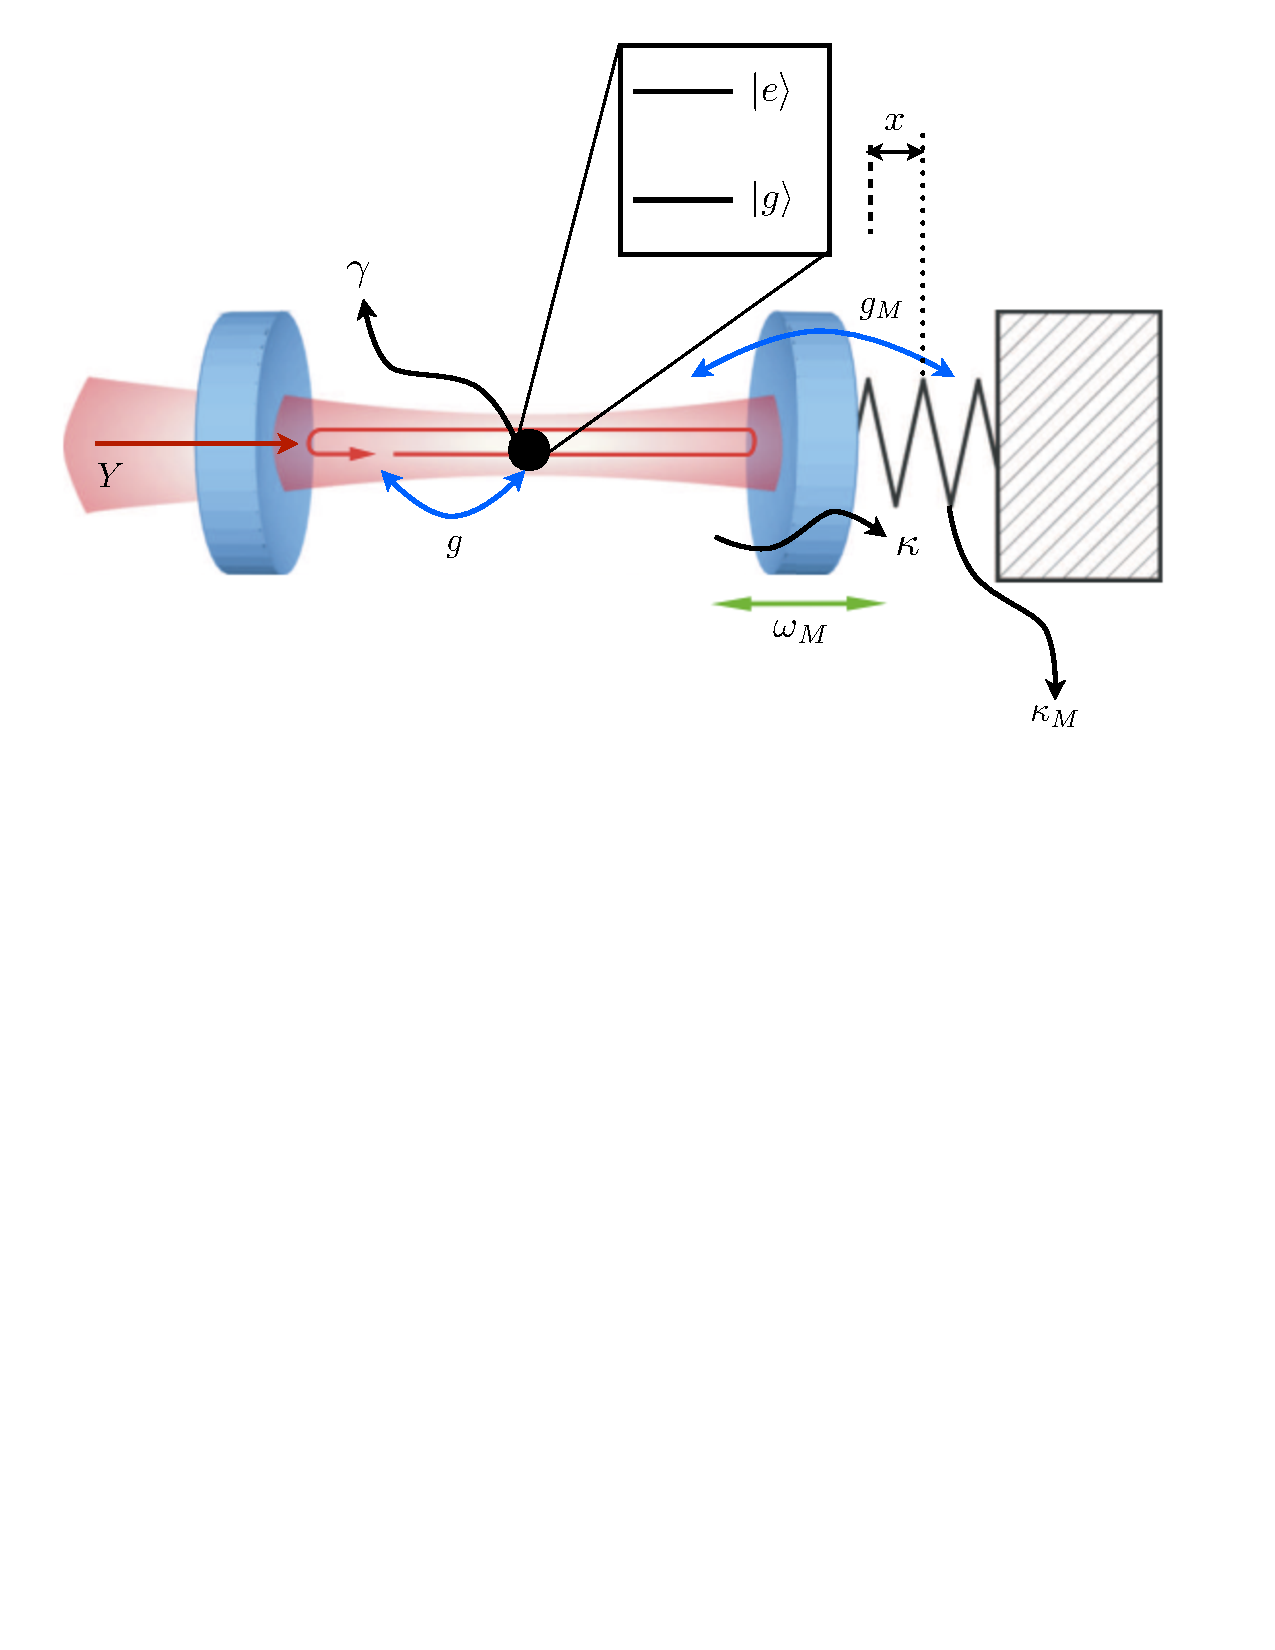
\includegraphics[width=0.7\textwidth]{Figures/1Apparatus}
\caption[A schematic of our imagined cavity optomechanics apparatus]{\small{A schematic of our imagined cavity optomechanics apparatus. The driving rate $Y$ is shown in red, while dissipative losses are drawn in black and coupling rates are blue. We also show the displacement of the oscillator, and length $L$ is the distance between the two end mirrors, which will oscillate in time.}}
\label{fig1Apparatus}
\end{center}
\end{figure}

We consider the apparatus of Fig.~\ref{fig1Apparatus} by starting with an optomechanical, non-Hermitian Hamiltonian demonstrating coupling between the cavity and oscillator that goes linearly with displacement. The method of quantum trajectory theory is implemented using the Quantum Toolbox in Python, or QuTiP \cite{qutipref}. The software is able to numerically calculate the state of the system and any stated expectation values over a range of times. With only slight adjustment, we can also calculate probe spectra and second-order correlation values. We plot various quantities and compare the results to what is expected from the Jaynes-Cummings cQED model. Ultimately, we aim to determine modifications due to the introduction of the mechanical oscillator.

\section{Outline of Thesis}
In chapter two, we detail the three primary theoretical frameworks used in this thesis. First, we derive the master equation in standard Lindblad form, detailing the various approximations made to achieve the form used. Second, we follow the approach of Carmichael and illustrate quantum trajectory theory, as well as explaining its advantage in QuTiP over the differential equation solver as applied to the Schr\"{o}dinger equation. Lastly, we explicitly write the Hamiltonian for the atom-field-oscillator system and detail the various parameters assigned to the mechanical spring. In chapter three, we treat the oscillator as a classical object, considering its dynamics when modeled as a harmonic oscillator and then when placed in a thermal state. Chapter four brings us to a fully quantum mechanical realization, and we determine probe spectra along with atom-field and field-field second-order correlations $g^{(2)}(0)$ and $g^{(2)}(\tau)$. Finally, in chapter five we summarize our results and point to future work for a weakly-driven optomechanical cavity with a two-level atom.